\documentclass{article}
\usepackage{amsmath, amssymb, enumitem}
\usepackage{geometry, graphicx, hyperref}

\geometry{margin=1in}
\begin{document}


\begin{center}

\section*{Desmos User Guide}
    
\end{center}

\begin{enumerate}
    \item \textbf{Entering Expressions}

    You can directly type mathematical expressions into Desmos without using a mouse or trackpad. For example:

    \[
    \frac{x^2}{3} \cdot \cos^2(x) + \sqrt{10x}
    \]

    \begin{center}
        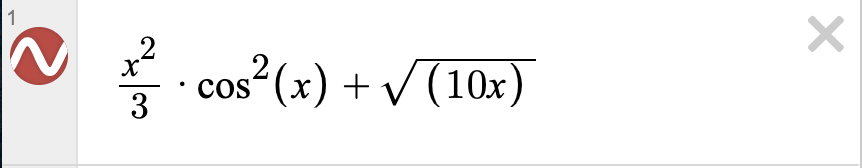
\includegraphics[width=0.8\linewidth]{E68.png}
    \end{center}

    \item \textbf{Switching Between Decimals and Fractions}

    Desmos allows you to convert decimal answers into fractions and vice versa. Just click the button that appears when a result can be represented both ways. For example:

      \begin{center}
        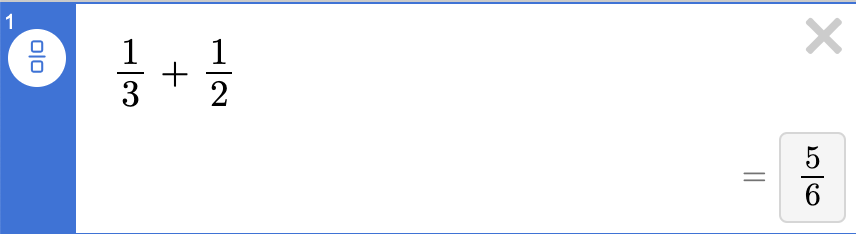
\includegraphics[width=0.8\linewidth]{E69.png}
    \end{center}

    \item \textbf{Graphing Equations Directly}

    You do not need to solve for \(y\) first. Simply type the equation as it is. For example:

      \begin{center}
        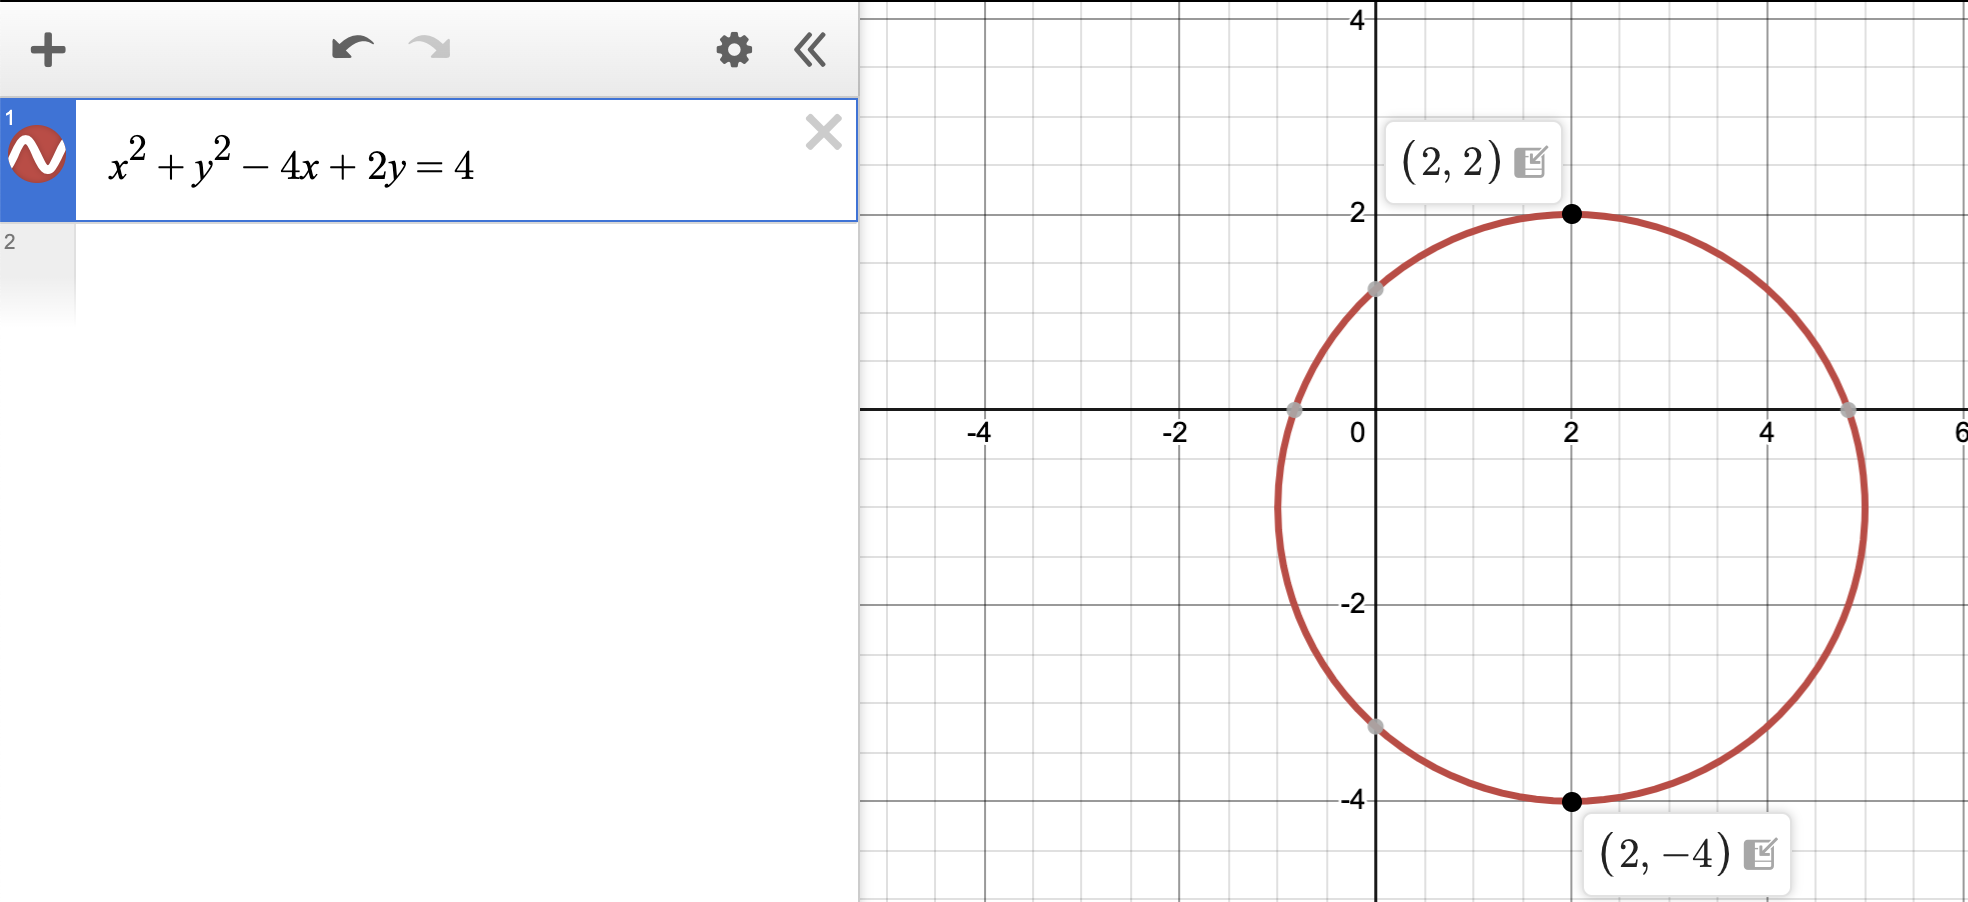
\includegraphics[width=1\linewidth]{E70.png}
    \end{center}

    Desmos will automatically graph the equation, including circles, ellipses, and other shapes.

    \item \textbf{Finding Solutions to Equations}

    You can enter an equation like:
      \begin{center}
        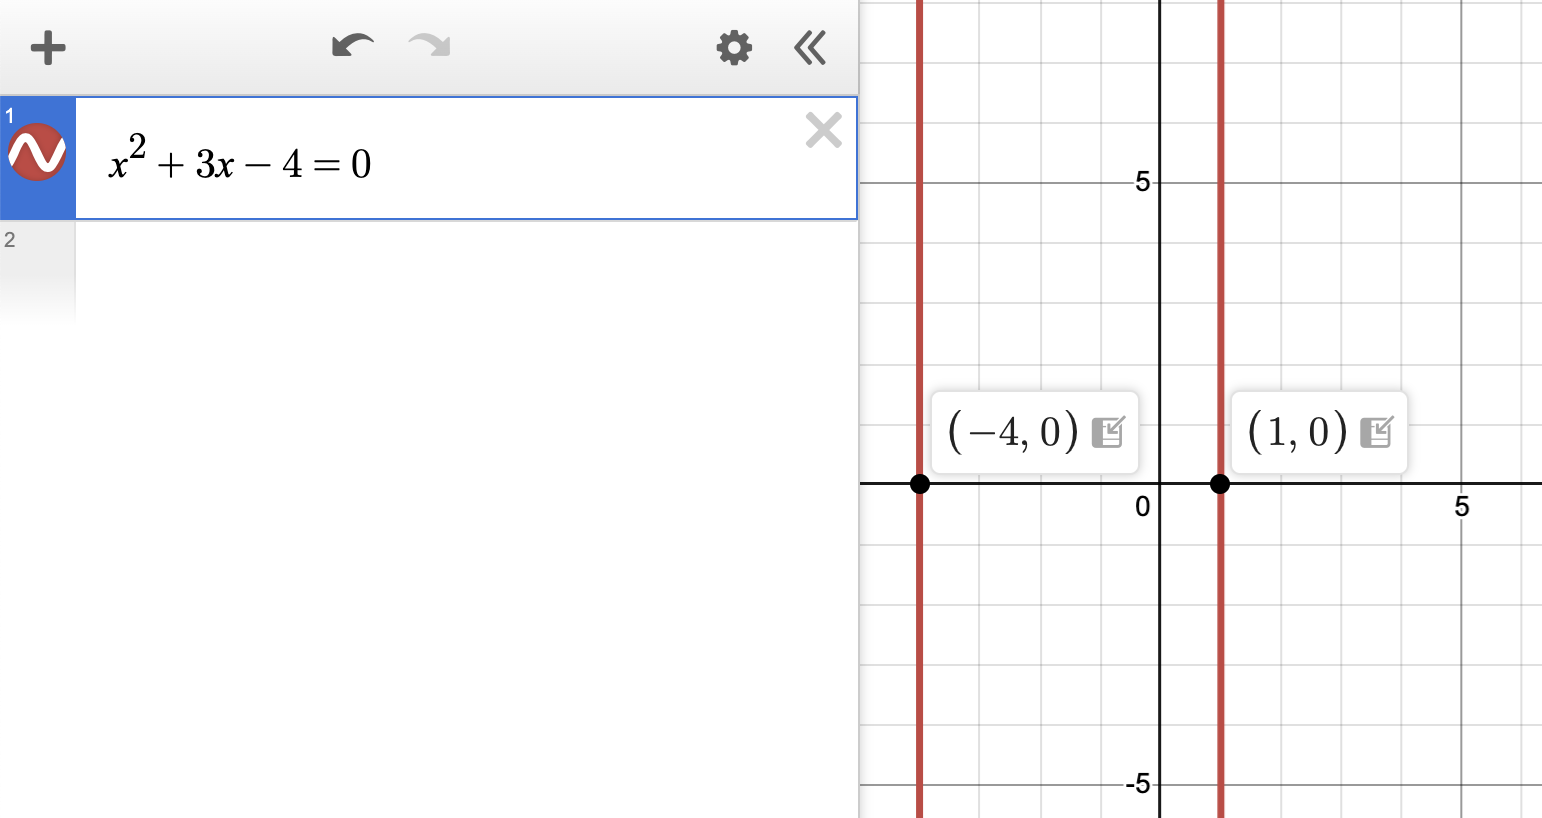
\includegraphics[width=1\linewidth]{E71.png}
    \end{center}

    Then click on the \(x\)-intercepts shown on the graph. Desmos will display the solutions at the intersection points.

    \item \textbf{Identifying Key Points}

    Desmos can highlight intersection points, \(y\)-intercepts, \(x\)-intercepts, maximums, and minimums. For example, enter:
          \begin{center}
        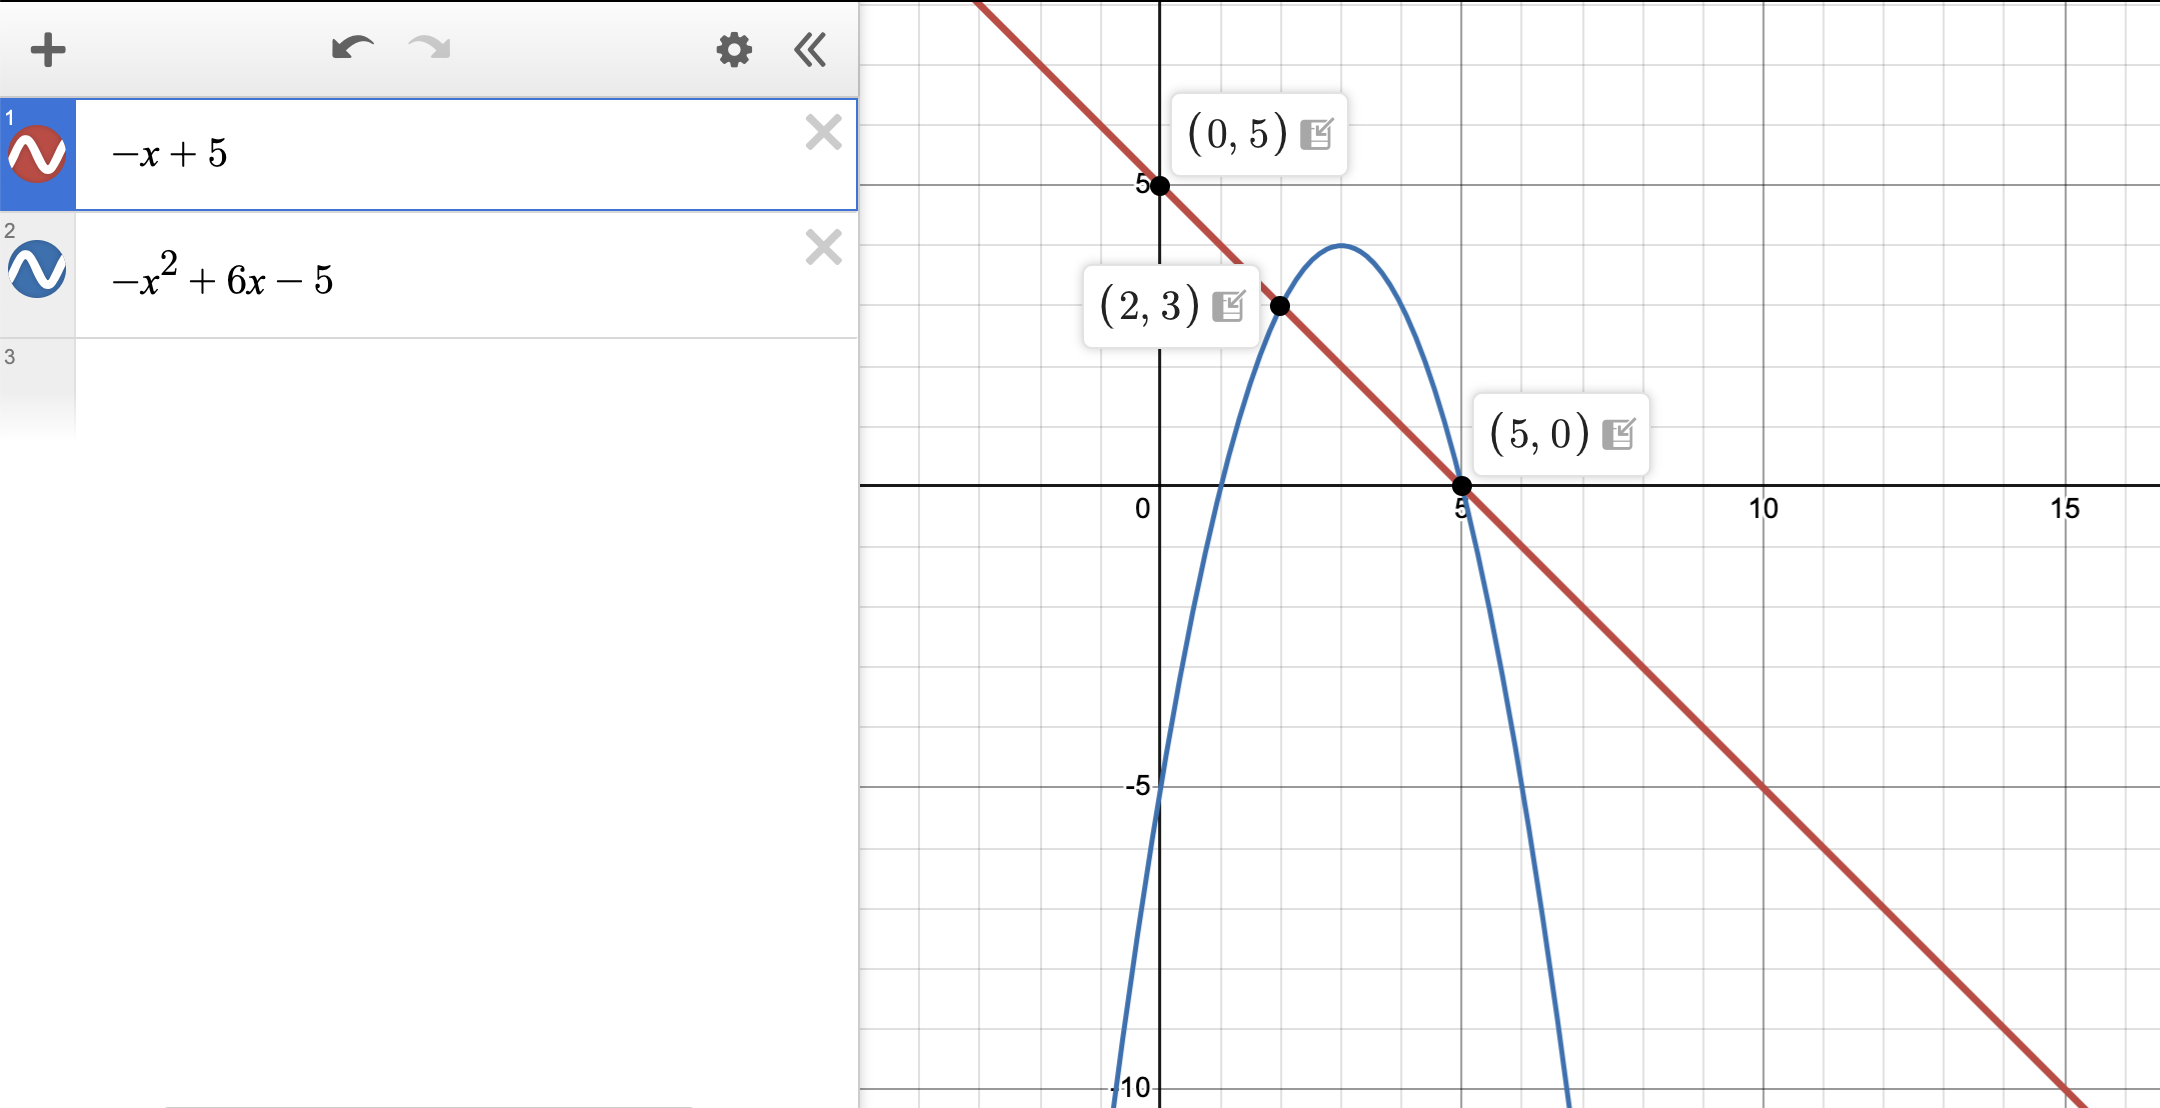
\includegraphics[width=1.1\linewidth]{E72.png}
    \end{center}


    Then click on the gray dots to view the coordinates of important points.

    \item \textbf{Performing Function Transformations}

    Desmos supports function notation and transformations. For example, defining:

    \[
    f(x) = x^2 - 4x + 3
    \]

    and translating it 2 units to the right gives:

    \[
    g(x) = f(x - 2)
    \]

    Desmos will display both functions for comparison.

    \item \textbf{Setting the Angle Unit}

    When performing trigonometric calculations, ensure the correct angle unit is selected—either radians or degrees.  
    You can change this setting by clicking the wrench icon in the upper right corner ("Graph Settings") and choosing \textbf{Radians} or \textbf{Degrees}.
\end{enumerate}
\end{document}